\begin{minipage}{.5\textwidth}
	\centering
	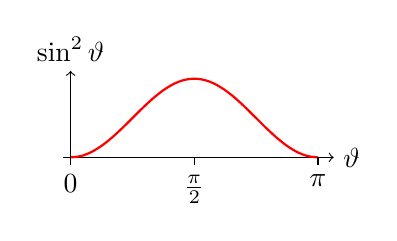
\begin{tikzpicture}
		\draw[->] (-.1, 0) -- (pi+0.2, 0) node[right] {$\vartheta$};
		\draw[->] (0, -0.1) -- (0, 1.1) node[above] {$\sin^2\vartheta$};
		\draw[domain=0:pi, smooth, variable=\x, red, thick] plot ({\x}, {(sin(\x*180/pi))^2});
		\draw[thin] (0,0) -- (0,-0.1) node[below]{$0$};
		\draw[thin] (pi/2,0) -- (pi/2,-0.1) node[below]{$\frac{\pi}{2}$};
		\draw[thin] (pi,0) -- (pi,-0.1) node[below]{$\pi$};
	\end{tikzpicture}
\end{minipage}
\begin{minipage}{.5\textwidth}
	\centering
	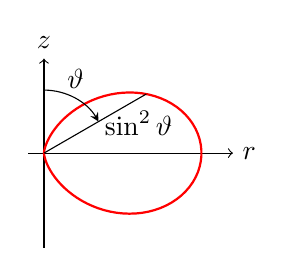
\begin{tikzpicture}[scale=2]
		\draw[->] (-.1, 0) -- (1.2, 0) node[right] {$r$};
		\draw[->] (0, -0.6) -- (0, 0.6) node[above] {$z$};
		% \draw[thick,red] (0,0) \foreach \th in {1, ... ,180} { -- ({90-\th}:{(sin(\th))^2}) };
		\draw[thick,red,variable=\th,domain=0:180,samples=90]
		plot ( {(sin(\th))^3} , {cos(\th)*(sin(\th))^2} );
		\draw [thin] (0,0) -- (30:{(sin(60))^2}) node[midway, right]{$\sin^2\vartheta$};
		\draw [thin,-stealth] (0,0.4) arc (90:30:0.4) node[midway,above]{$\vartheta$};
	\end{tikzpicture}
\end{minipage}